\documentclass[11pt, A4paper, english]{article}
\usepackage{amsfonts}
\usepackage{amsmath}
\usepackage{amssymb}
\usepackage{amsthm}
\usepackage{babel}
\usepackage{caption}
\usepackage{color}
\usepackage{float}
\usepackage[T1]{fontenc}
\usepackage[a4paper, total={18.5cm, 24cm}]{geometry}
\usepackage{graphicx}
\usepackage[colorlinks]{hyperref}
\usepackage[utf8]{inputenc}
\usepackage{listings}
\usepackage{textcomp}
\usepackage[style=ieee]{biblatex}
\usepackage{tabularx}
\usepackage{multicol}

\addbibresource{bibliography.bib}

\definecolor{url}{rgb}{0.1, 0.1, 0.4}

\lstset{frame=tb,
	language=csh,
	aboveskip=3mm,
	belowskip=3mm,
	showstringspaces=false,
	columns=flexible,
	basicstyle={\small\ttfamily},
	numbers=none,
	breaklines=true,
	breakatwhitespace=true,
	tabsize=3
}

\textwidth = 530pt

\lstset{inputpath="C:/Users/Torstein/Documents/skole/USN/IIA2017/Assignment 6"}
\graphicspath{{C:/Users/Torstein/Documents/USN/IIA2017/Assignment 6/}}
\hypersetup{colorlinks = true, linkcolor = black, urlcolor=url}

\renewcommand{\thefigure}{\arabic{section}.\arabic{figure}}
\renewcommand{\thetable}{\arabic{section}.\arabic{table}}
\numberwithin{equation}{section}

\author{Torstein Solheim Ølberg \\
	University of South-Eastern Norway}
\title{SCADA System for Air Heater}



%\lstinputlisting{Filnavn! type kodefil}. Use [linerange=0-73] or [linerange=73-] to crop
%\includegraphics[width=12.6cm, height=8cm]{Filnavn! type png}



\begin{document}
	\maketitle
	
	\begin{multicols}{2}
		\section*{Abstract}
Last winter, contest was posted to do something with their inadequate heating system and the development for a new heating system begun. The heating system, built up like a SCADA system consists of an air heater, a controller and DAQ application, an OPC UA server, a data logging program, an SQL database and a display and alarm application. Since the hardware for the system has not arrived yet, the system was developed using a simulation of the air heater which was tuned using a borrowed real heater. The finale product is capable of controlling and logging the temperature, but should be tested with the hardware when this arrives. \\
\newline
\textbf{Keyword:} \textit{Heater, SCADA, LabVIEW, WindowsForms, Simulation}

		\section{Introduction}
During the winter of 2024, the company MadeUpCompany AS experienced that their heating system was unable to keep up with the fall in temperature. As a result, a new air heater system must be installed, adding to the system already in effect. To help with this, a contest was announced to develop a prof of concept SCADA (Supervisory Control And Data Acquisition) system capable of heating the air, measuring the temperature of the environment and alert the users if the temperature is outside the comfortable range. MyCompany AS has decided to enter the competition, and the general structure of the product to be developed can be seen if figure \ref{fig:system_sketch}. This system includes heaters connected to individual controllers via cable sending signals between them. The controllers also communicate via a local network to a database which stores the temperature data and communicates via a local network with a desktop displaying the statistics of the process live. As the hardware for the system has not arrived yet, a simulating setup of the system was produced. Only a single heater simulator, controller and server is possible to begin with due to this shortage in hardware, but this can be extended later to cover an entire workplace. \\
			\begin{figure}[H]
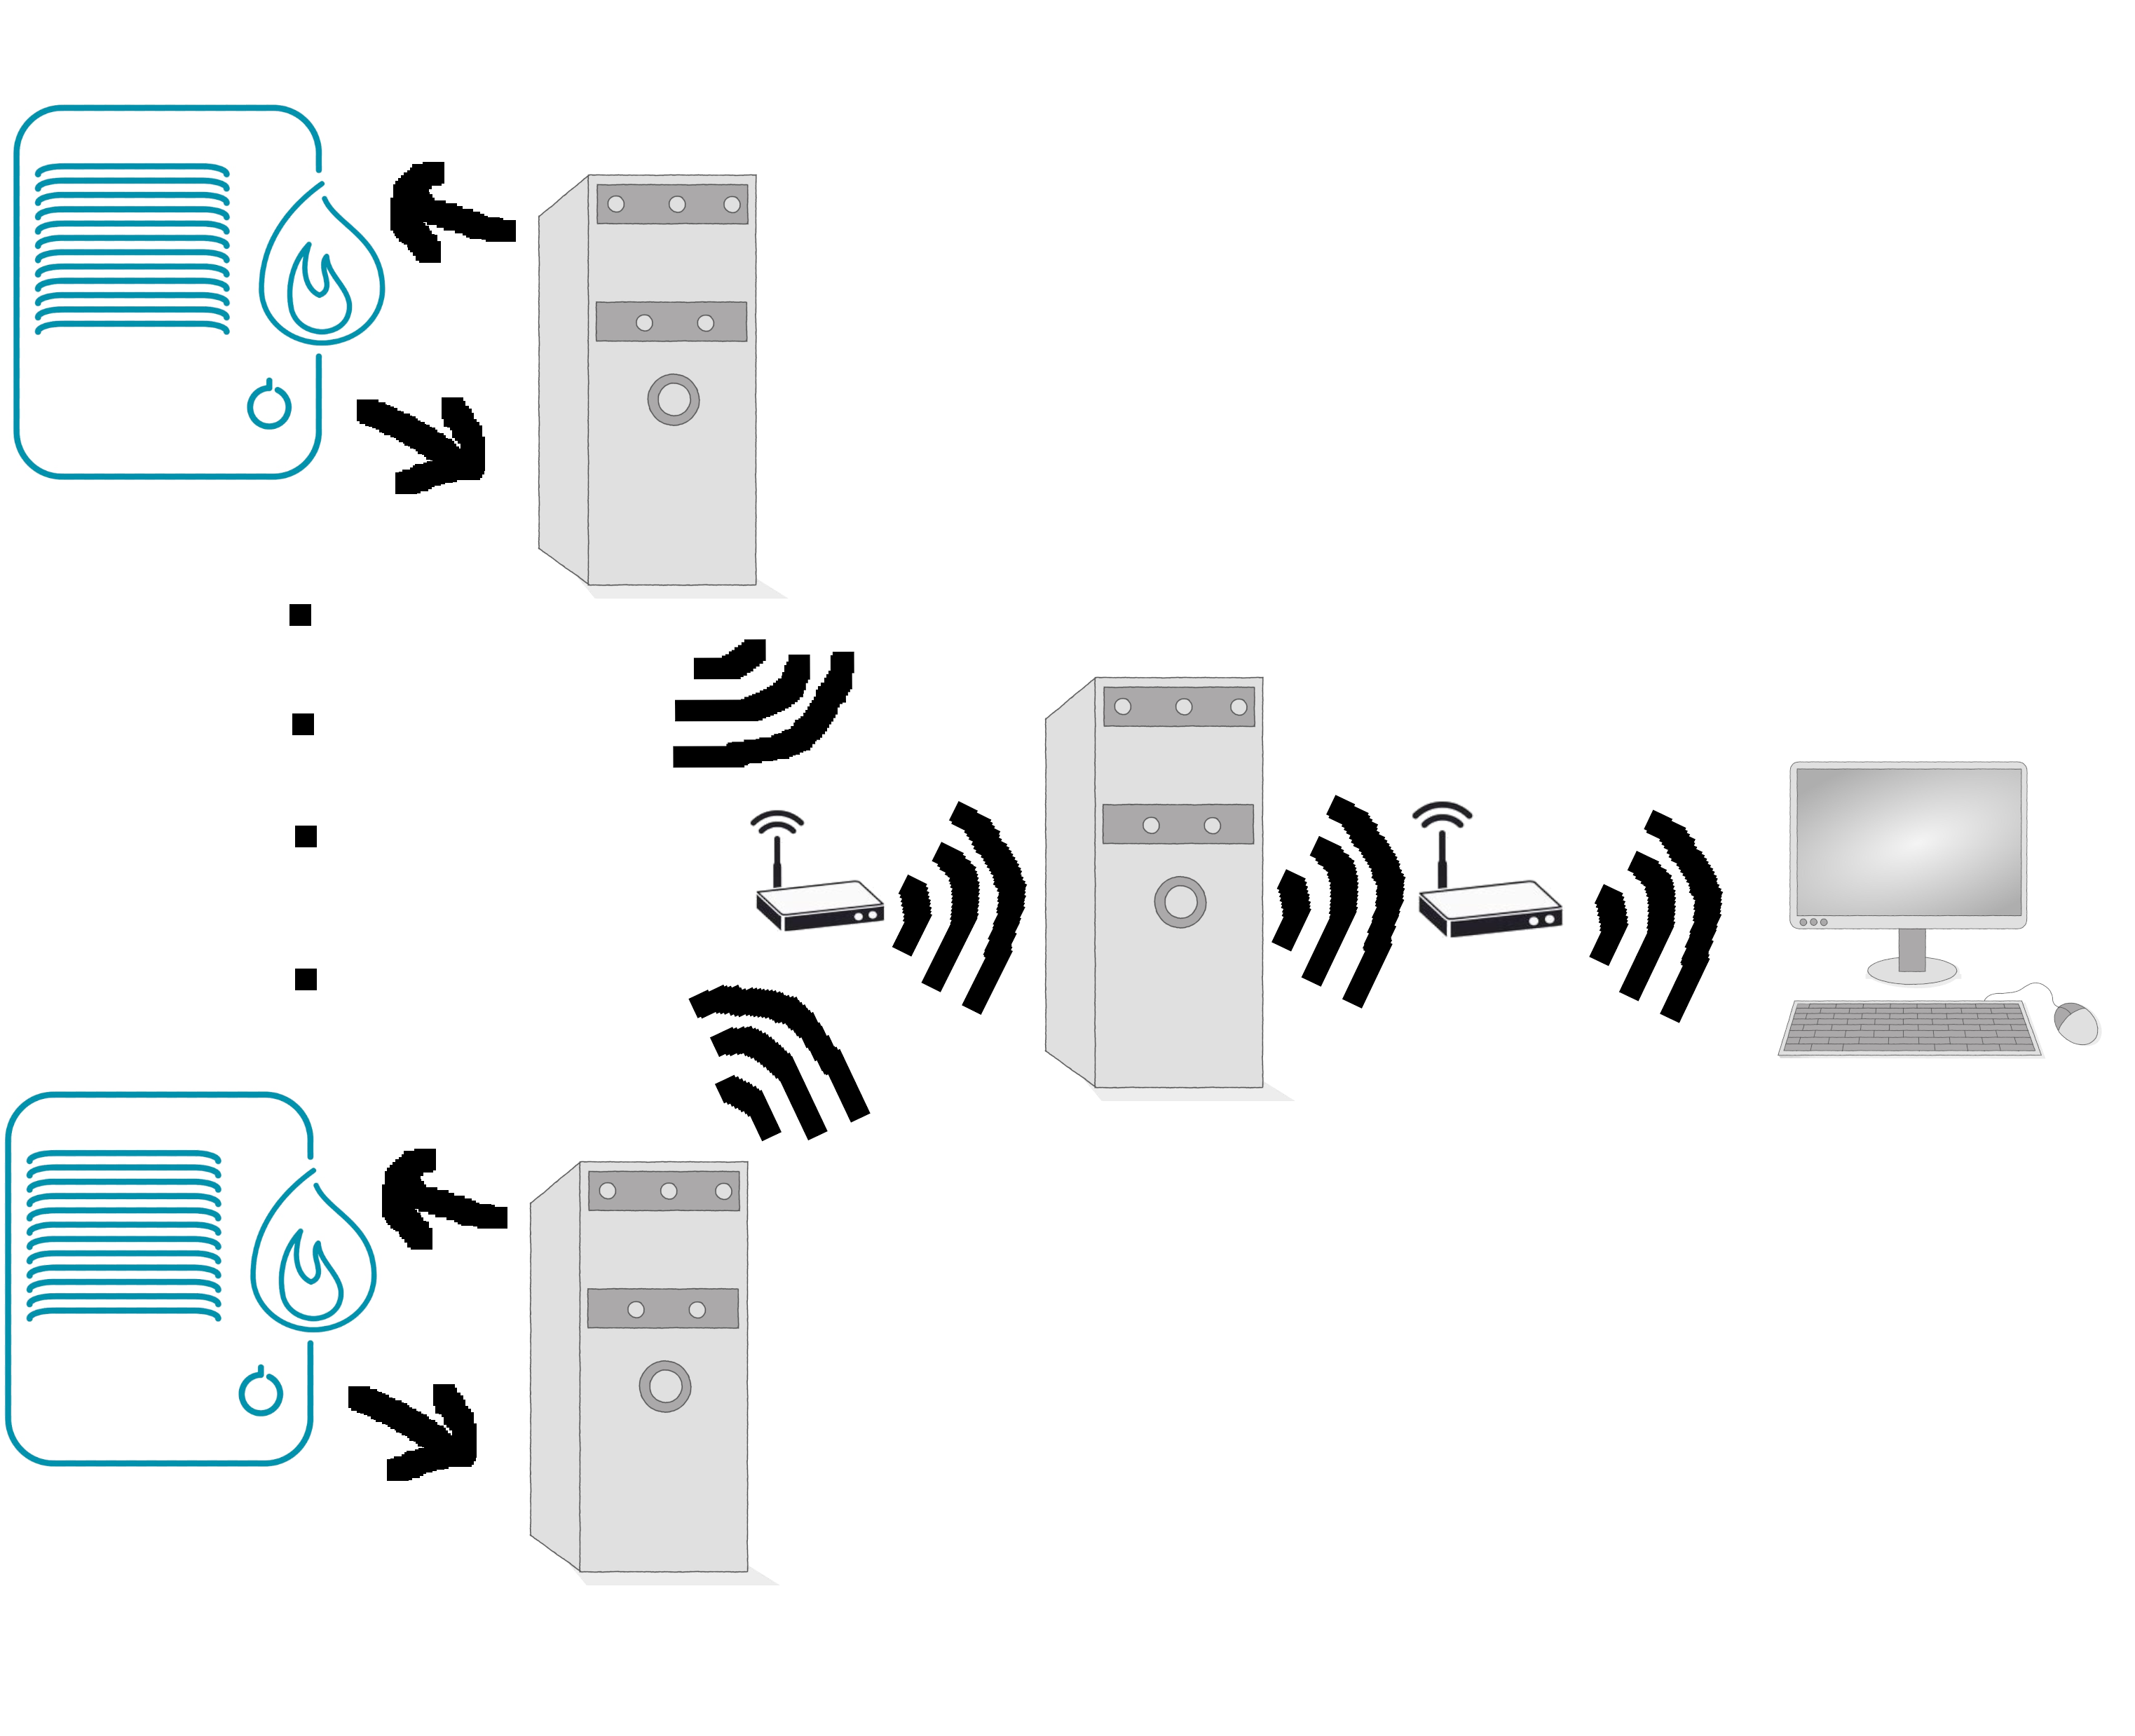
\includegraphics[width=\columnwidth]{SCADA_sketch.png}
\caption{SCADA system sketch. Heaters and their controllers interact through cable while the database interacts with the controllers and display system wirelessly through a local network.}
\label{fig:system_sketch}
			\end{figure}
This report will outline the process which was done to create this system. First, the methods and tools used to develop the system will be presented. Then, the system will be presented, along with the most important parts of the code and the results of testing it. Finally, the usefulness of the system and its capability to solve the problem will be discussed and a conclusion will be drawn.
		
		\section{Materials and Methods}
The Method section will outline the tools and methods used for development of the system. Each subsection will present a different set of tools and how they where used in this project.
		
		\subsection{Air heater}
The heater which has been ordered for use in the system is the same one presented by Haugen \cite{airheater}. It consists of a fan which sucks in air, a heater controller taking in an electric signal between zero and five volt, and a temperature sensor which gives of a one to five volt electrical signal corresponding to between zero and 50 degrees Celsius. Since this heater is not available yet, a simulated heater model \cite{airheatermodel} has been used instead. This air heater model must be tuned for the purpose of acting similar to its real life counterpart, which was done by travelling to the manufacturer of the heater and borrowing a heater. \\
The simulator needs to be given a set of parameters to work, and these are the once to tune such that the simulated air heater acts like a real one. These parameters are a presented by Haugen \cite{airheater}, and include the environment temperature, heat gain per volt, time delay and response time. When tuned, the simulator was used just like the air heaters will be used for the remaining development.

		\subsection{LabVIEW}
For multiple parts of the software development process, the development platform LabVIEW \cite{LabVIEW} was used as a tool to construct simple programs running on a Windows machine. A 32 bit 2023 Q3 version for Windows was used. This is a visual programming language where both the design of the frontend display and the backend logic is done simultaneously. For development of the controller and OPC UA applications, the two add-on packages NI-DAQmx and NI LabVIEW OPC UA Toolkit where also used.
		
		\subsection{Controller}
The controller was developed, using LabVIEW, as a PID (proportional Integral Derivative) controller coded in a formula node. The equations describing the behaviour of the controller are equations \ref{eq:P}, \ref{eq:I}, \ref{eq:D} and \ref{eq:PID}.
			\begin{equation}
u_P = K_P \cdot e_i
\label{eq:P}
			\end{equation}
			\begin{equation}
u_I = u_{i - 1} + K_i \cdot dt \cdot e_i
\label{eq:I}
			\end{equation}
			\begin{equation}
u_D = K_D \cdot \frac{e_i - e_{i - 1}}{dt}
\label{eq:D}
			\end{equation}
			\begin{equation}
u_i = u_P + u_I + u_D
\label{eq:PID}
			\end{equation}
Here $u_i$ is the controller signal sent out by the controller, $u_{i - 1}$ is the previous control signal, the different K values are tuning parameters for the controller, the e values are the difference between the measured temperature and the optimal temperature for the current and previous calculation, and the dt is the time step since the last signal. Since the range of controller signals only goes from zero to five volt, a check restricting the signal from over or under shooting this range was implemented. \\
A problem with the PID controller, especially due to the derivative term $u_D$, is its vulnerability to noise in measurements and instability when reacting quickly. For this purpose, a low pass MA (Moving Average) filer was implemented to help average out any instability. The MA filter used was described by Haugen \cite{MA} in equation 1.10 and 1.11, but can also be seen in equation \ref{eq:MA}.
			\begin{equation}
y_{i, f} = y_{i - 1} + \frac{(y_i - y_{i - 1}) dt}{T_w + dt}
\label{eq:MA}
			\end{equation}
The filtered value is given by the current and previous values $y_i$ and $y_{i - 1}$ along with a time step between the signals $dt$ and a time window the filter should average over $T_w$. \\
After the MA filter was added, the controller was tuned using the Ziegler-Nichols closed loop method described by Haugen \cite{MA}, but as these values gave a very slow reacting controller, the values where adjusted manually afterwards.
The controller, along with a display logging the live data of the temperature and the signal from the controller was built into a program running in a loop until a stop button is pressed. A timer showing the time since the start of the program, and a set of tabs for controlling the controller and air heater model is also included.
		
		\subsection{OPC UA Server}
To communicate between the controller and the database, an OPC UA server was developed, with the simple ability to store to nodes of data. The server was developed using LabVIEW OPC UA Toolkit and stores a single data point value and the location it was acquired at, to be read by a OPC UA client and passed on to a database storage. \\
A pair of OPC UA clients, one for reading from and one for writing to the server where also made using the toolkit. The writer is used by the controller to pass data to the server, while the reader is used by the SQL server writer.
		
		\subsection{SQL Server}
An SQL server database was set up using Microsoft SQL Server \cite{SQL} and designed using erwin Data Modeler \cite{erwin}. erwin Data Modeler is a graphical database design tool used to produce diagrams for an code to set up a general framework for a database. SQL is a database language used for setting up tables and functions where data can be stored and extracted. In this, the database stores data points from the OPC UA server using the OPC UA reader client and a LabVIEW program connecting to the SQL server and writing the temperature value to a data point table along with a corresponding location. The data point table stores the data value, its location reference, the unit Celsius and the time it was logged. This program also displays the location and data logged. A table using SQL to calculate a set of statistics for each location, including the min and max temperature values, and the mean and standard deviation values, was also added.
		
		\subsection{Visual Studio, Windows Forms and The Display Application}
To display the data stored in the SQL server, a Windows Forms application was developed to allow the program to run on more than just windows operating systems. Windows Forms applications are a type of .NET applications developed using C\#. In this project, the development platform Microsoft Visual Studio \cite{VS} was used with the added NuGet packages Microsoft.Data.SQLClient 5.2.0 \cite{SQLClient} and ScottPlot/ScottPlot.WinForms 5.0.34 \cite{ScottPlott} to design the frontend and code the back end of the display application, and to add functionality for it to send an email to a user specified email address if temperature ranges outside a comfortable interval.

		\section{Results}
In this section the resulting applications developed will be presented. All code an applications can be found on the github page of the project as well \cite{github}. 
			
			\subsection{DAQ}
				\subsubsection{Air Heater Model}
The tuned air heater model performance compared to the actual data from the borrowed heater can be seen in figure \ref{fig:tuned}.
				\begin{figure}[H]
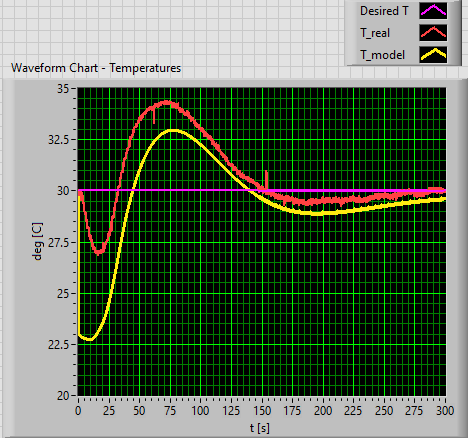
\includegraphics[width=\columnwidth]{Tuned model with filter data.png}
\caption{Tuned air heater model alongside real data.}
\label{fig:tuned}
				\end{figure}
The two curves follow the same general movement with a minor difference in the starting point and stability. The model displayed has the parameters shown in table \ref{tab:model parameters}.
				\begin{table}[H]
\caption{The air heater model parameters after tuning.}
		\noindent \begin{tabularx}{\columnwidth}{@{}l | l}
\hline
\textbf{Model Parameters}	\hspace{2cm}	& \textbf{Values}	\\
\hline
Initial Temp 								& 22 [C] 			\\
Heat Gain 									& 3.2 [C/V]			\\
Time Constant								& 5.5 [s]			\\
Time Delay									& 3 [s]	 			\\
Initial Time Delay						 	& 0	[s]				\\
Maximum Time Delay						 	& 5 [V]				\\
Environment Temp			 				& 22 [C]			\\
\hline
					\end{tabularx}
\label{tab:model parameters}
				\end{table}
			
			\subsubsection{Controller}
The parameters after tuning the controller can be seen in table \ref{tab:controller parameters}.
				\begin{table}[H]
\caption{The air heater controller parameters after tuning.}
		\noindent \begin{tabularx}{\columnwidth}{@{}l | l}
\hline
\textbf{Model Parameters}	\hspace{2cm}	& \textbf{Values}	\\
\hline
Proportional Gain ($K_P$)  					& 0.06 				\\
Integral Gain ($K_I$)						& 0.3				\\
Derivative Gain	($K_D$)						& 0.3				\\
\hline
					\end{tabularx}
\label{tab:controller parameters}
				\end{table}

			\subsubsection{Complete application}
The finale application is a program which, as shown in figure \ref{fig:daq}, can run a simulation of the air heater model and log the data of the controller signal and temperature to their own displays. Further more, the application also writes the data and a location to an OPC UA Server and displays the run time of the program.
				\begin{figure}[H]
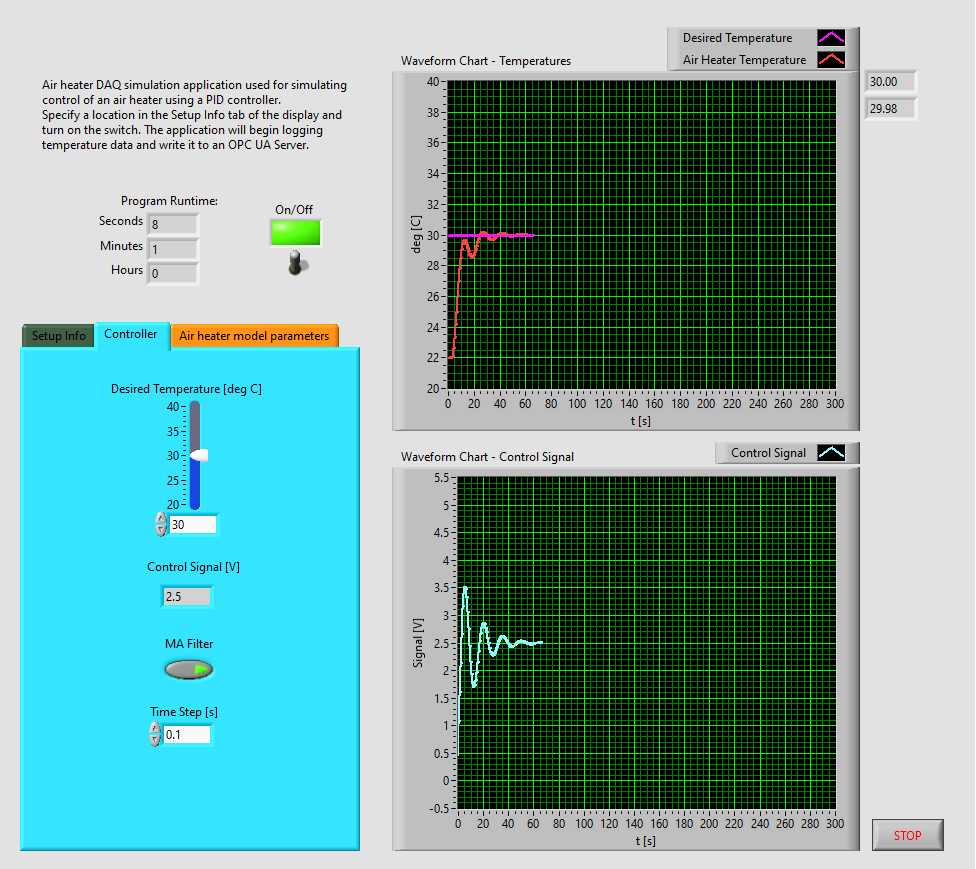
\includegraphics[width=\columnwidth]{DAQ.png}
\caption{The DAQ application photographed during runtime}
\label{fig:daq}
				\end{figure}
		
		\subsection{OPC UA Server}
The OPC UA Server, shown in figure \ref{fig:opc-server}, runs until stopped and simply holds the data values of the temperature and location to be written to or read from.
			\begin{figure}[H]
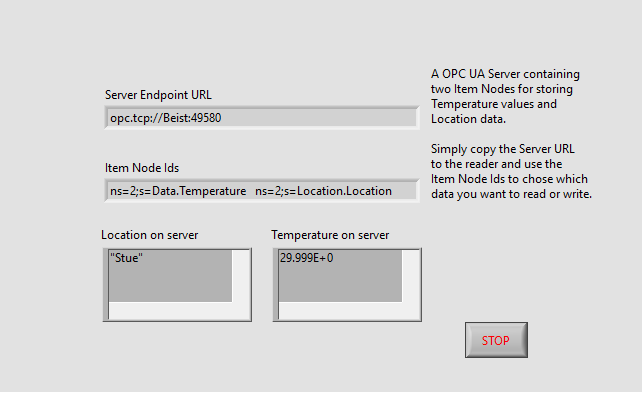
\includegraphics[width=\columnwidth]{OPC Server.png}
\caption{Image of the OPC UA server while running. The address of the server and the ids of the two nodes are visible along with the current value of the nodes.}
\label{fig:opc-server}
			\end{figure}
		
		\subsection{SQL Database and Data Logger Application}
The data logging application for the SQL database can be seen in figure \ref{fig:datalogger}.
			\begin{figure}[H]
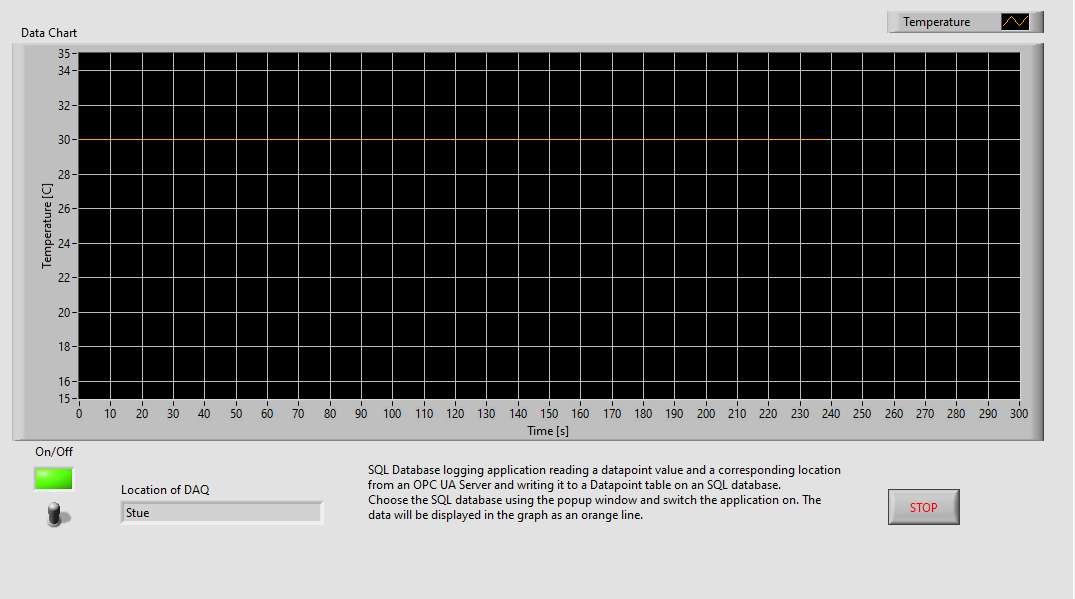
\includegraphics[width=\columnwidth]{Datalogger.png}
\caption{Image of the data logging application while running.}
\label{fig:datalogger}
			\end{figure}
It shows a graph displaying the values of the OPC UA server and the location on the server. As the value of the graph is constant at 30 Celsius since the server is not written to. Meanwhile, the application is writing data to the SQL database shown in figure \ref{fig:SQL diagram}.
				\begin{figure}[H]
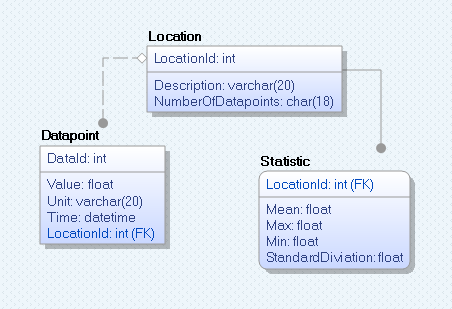
\includegraphics[width=\columnwidth]{Diagram.png}
\caption{Diagram of the SQL server.}
\label{fig:SQL diagram}
				\end{figure}
This is an SQLEXPRESS Server database called Temperature Logging and Control System. \\
The data logging and alarm application is the finale part of the system, and can be seen in figure \ref{fig:display-and-alarm-system}. The application is display showing the data on the database live for a single location. In the settings tab, the database and location can be changed. The update interval for the application and the alarm email used if the detected temperature is above or below comfortable levels can also be set.Finally, there is a help tab with instructions on how to use the program.
				\begin{figure}[H]
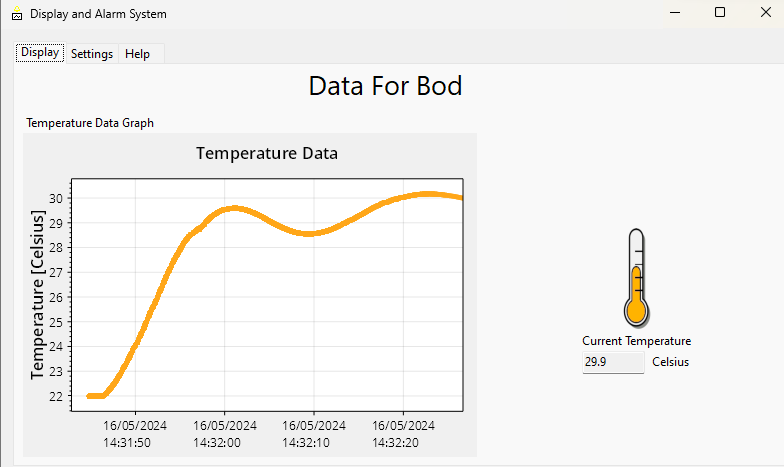
\includegraphics[width=\columnwidth]{Display and Alarm System.png}
\caption{Data logging and alarm application while running.}
\label{fig:display-and-alarm-system}
				\end{figure}
				\begin{figure}[H]

\includegraphics[width=\columnwidth]{Alarm.png}
\caption{An alarm emailed to a user when temperature exceeds 30 degrees Celsius.}
\label{fig:alarm}
				\end{figure}
In figure \ref{fig:alarm} there is an image proving an alarm was sent when the program running in figure \ref{fig:display-and-alarm-system} hit above 30 degrees Celsius. \\

			\subsection{Complete System}
The completed system was tested and this run can be seen in figure \ref{fig:complete}.
				\begin{figure}[H]
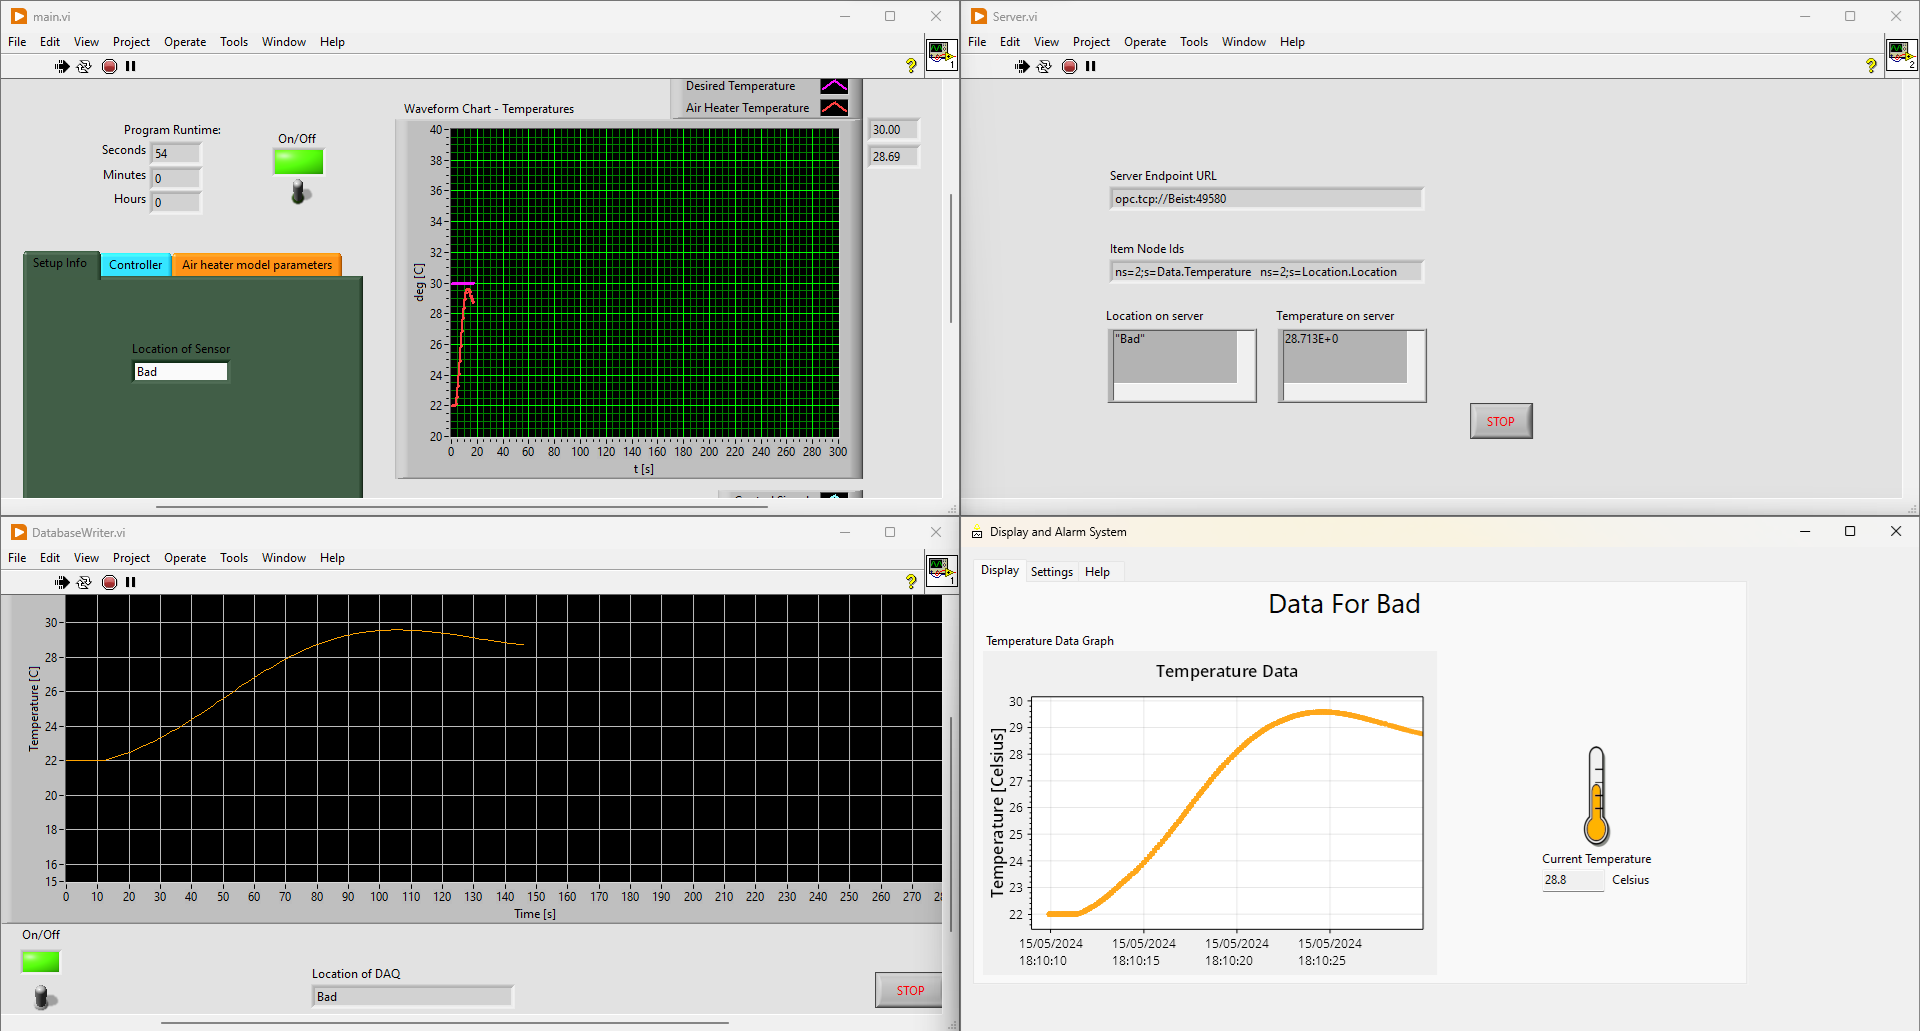
\includegraphics[width=\columnwidth]{Complete Setup.png}
\caption{Running the complete system. All parts of the application interact with each other producing the same data.}
\label{fig:complete}
				\end{figure}
The finale system runs smoothly with all parts interacting at the same machine. The system has also been tested at worked seamlessly with the display and alarm application running on a different Windows machine.

		\section{Discussion}
This section discusses the system with regard to its fulfilment of the original specification and any future improvements upon the work. \\
The finale application has been shown to be able to control a simulated air heater system and save the measured temperature data to a database. Then it can display this data on a different computer and the user can be notified if the temperature is to high or to low. This was the function of the SCADA system and what the original specifications stated, since the controller and measuring device has been shown to also be able to work with a real heater. However, As the system is now, most of the applications are only capable of interacting with specific other systems, and a more flexible UI option should be included. The DAQ and data logging applications should have options for selecting user defined OPC UA servers. This is not really necessary due to the system being developed to work with each other, but would help with later development if the system is to be extended. The system must however also be tested with the correct hardware setup when this arrives, to confirm the OPC client on the controller is capable of communicating with the database through the local network. Finally, since the system communicates through a local network, there is a risk of the data being collected by a potential hacker, which could log the data or attempt to sabotage the system by sending unwanted settings to the controller and then overloading the system with request. To combat this, a possibility to force a login when interacting with the OPC server, and also an encryption of the data sent over the local network would be a good idea.
		
		\section{Conclusion}
A Temperature logging and control SCADA system has been developed for the competition posted by MadeUpCompany AS and the system has been tested such that it should be operational as soon as the hardware arrives. The system consists of a controller and DAQ program, an air heater, an OPC UA server, a data logging application, an SQL server and a display and alarm system. The finale product works fine as is, but could be improved upon for later extension and should be tested to check if finished when the finale hardware is acquired.
		
\printbibliography
		
	\end{multicols}
\end{document}
